
C++20前,erase-remove通常用于从STL容器中删除元素。这操作有点麻烦,通常使用这样的函数来完成:

\begin{lstlisting}[style=styleCXX]
template<typename Tc, typename Tv>
void remove_value(Tc & c, const Tv v) {
	auto remove_it = std::remove(c.begin(), c.end(), v);
	c.erase(remove_it, c.end());
}
\end{lstlisting}

std::remove()函数在<algorithms>头文件中声明。remove()搜索指定的值,并将元素从容器的末尾向前移动来删除它,所以并不会改变容器的大小。它返回一个超出移位范围末端的迭代器,然后调用容器的erase()函数删除剩余的元素。

有了新的擦除功能,这个两步过程可以简化为一步:

\begin{lstlisting}[style=styleCXX]
std::erase(c, 5); // same as remove_value() function
\end{lstlisting}

这个函数与上面的remove\_value()函数功能相同。

还有一个版本使用了谓词函数。例如,要从数值容器中删除所有偶数值:

\begin{lstlisting}[style=styleCXX]
std::erase_if(c, [](auto x) { return x % 2 == 0; });
\end{lstlisting}

\subsubsection{How to do it…}

擦除函数有两种形式。第一种形式叫做erase(),有两个参数,一个容器和一个值:

\begin{lstlisting}[style=styleCXX]
erase(container, value);
\end{lstlisting}

容器可以是顺序容器(vector, list, forward\_list, deque),数组除外,数组不能改变大小。

第二种形式称为erase\_if(),接受一个容器和一个谓词函数:

\begin{lstlisting}[style=styleCXX]
erase_if(container, predicate);
\end{lstlisting}

这种形式适用于使用erase()的容器,也适用于关联容器、set、map及其多键和无序的版本。

函数erase()和erase\_if()作为非成员函数定义在相应容器的头文件中。

来看一些例子:

\begin{itemize}
\item 
首先,定义一个简单的函数来打印顺序容器的大小和元素:

\begin{lstlisting}[style=styleCXX]
void printc(auto & r) {
	cout << format("size({}) ", r.size());
	for( auto & e : r ) cout << format("{} ", e);
	cout << "\n";
}
\end{lstlisting}

printc()函数使用C++20的format()函数为cout格式化字符串。

\item 
下面是一个包含10个整数元素的vector,用printc()函数打印出来:

\begin{lstlisting}[style=styleCXX]
vector v{ 1, 2, 3, 4, 5, 6, 7, 8, 9 };
printc(v);
\end{lstlisting}

输出为:

\begin{tcblisting}{commandshell={}}
size: 10: 0 1 2 3 4 5 6 7 8 9
\end{tcblisting}

可以使用erase()删除所有值为5的元素:

\begin{lstlisting}[style=styleCXX]
erase(v, 5);
printc(v);
\end{lstlisting}

输出为:

\begin{tcblisting}{commandshell={}}
size: 9: 0 1 2 3 4 6 7 8 9
\end{tcblisting}

std::erase()函数的vector版本定义在<vector>头文件中。在erase()调用之后,删除值为5的元素,vector中有9个元素。

\item 
这也适用于列表容器:

\begin{lstlisting}[style=styleCXX]
list l{ 0, 1, 2, 3, 4, 5, 6, 7, 8, 9 };
printc(l);
erase(l, 5);
printc(l);
\end{lstlisting}

输出为:

\begin{tcblisting}{commandshell={}}
size: 10: 0 1 2 3 4 5 6 7 8 9
size: 9: 0 1 2 3 4 6 7 8 9
\end{tcblisting}

std::erase()函数的列表版本定义在<list>头文件中。erase()之后,删除值为5的元素,list有9个元素。

\item 
erase\_if()可以使用一个简单的谓词函数,删除所有偶数元素:

\begin{lstlisting}[style=styleCXX]
vector v{ 0, 1, 2, 3, 4, 5, 6, 7, 8, 9 };
printc(v);
erase_if(v, [](auto x) { return x % 2 == 0; });
printc(v);
\end{lstlisting}

输出为:

\begin{tcblisting}{commandshell={}}
size: 10: 0 1 2 3 4 5 6 7 8 9
size: 5: 1 3 5 7 9
\end{tcblisting}

\item 
erase\_if()函数也适用于关联容器,比如map:

\begin{lstlisting}[style=styleCXX]
void print_assoc(auto& r) {
	cout << format("size: {}: ", r.size());
	for( auto& [k, v] : r ) cout << format("{}:{} ",
		k, v);
	cout << "\n";
}

int main() {
	map<int, string> m{ {1, "uno"}, {2, "dos"},
		{3, "tres"}, {4, "quatro"}, {5, "cinco"} };
	print_assoc(m);
	erase_if(m,
		[](auto& p) { auto& [k, v] = p;
		return k % 2 == 0; }
	);
	print_assoc(m);
}
\end{lstlisting}

输出为:

\begin{tcblisting}{commandshell={}}
size: 5: 1:uno 2:dos 3:tres 4:quatro 5:cinco
size: 3: 1:uno 3:tres 5:cinco
\end{tcblisting}

因为map的每个元素都是成对返回的,所以需要不同的函数来打印。print\_assoc()函数的作用:在for循环中使用结构化绑定来解包对元素。还可以在erase\_if()的谓词函数中使用结构化绑定,来隔离用于过滤偶数元素的键值。
\end{itemize}

\subsubsection{How it works…}

erase()和erase\_if()函数只是一次性执行erase-remove的包装器:

\begin{lstlisting}[style=styleCXX]
template<typename Tc, typename Tv>
void remove_value(Tc & c, const Tv v) {
	auto remove_it = std::remove(c.begin(), c.end(), v);
	c.erase(remove_it, c.end());
}
\end{lstlisting}

若考虑一个简单的int vector,称为vec,具有以下值:

\begin{lstlisting}[style=styleCXX]
vector vec{ 0, 1, 2, 3, 4, 5, 6, 7, 8, 9 };
\end{lstlisting}

可以将vec可视化为一行的int值表:

\hspace*{\fill} \\ %插入空行
\begin{center}
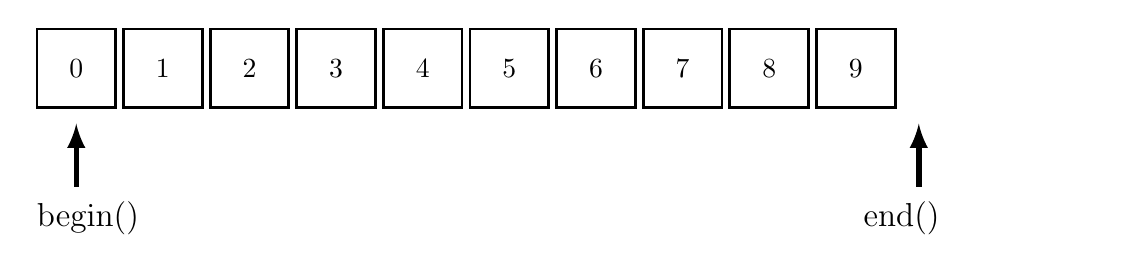
\begin{tikzpicture}
\foreach \x in {0,...,9} {
	\draw[line width=1pt] (1.1*\x,1) rectangle (1.1*\x+1,0) node[pos=.5] {\x};
}

\draw[line width=2pt][-latex] (0.5,-1.0) -- (0.5,-0.2);
\draw[line width=2pt][-latex] (11.2,-1.0) -- (11.2,-0.2);

\node[text width=3cm, font=\large] at (1.5,-1.4) {begin()};
\node[text width=3cm, font=\large] at (12,-1.4) {end()};
\end{tikzpicture}

图3.1  begin()和end()迭代器
\end{center}

begin()迭代器指向第一个元素,end()迭代器指向最后一个元素。此配置是所有STL顺序容器的标准。

使用remove(c.begin(),c.end(),5)时,算法从begin()迭代器开始搜索匹配的元素。对于找到的每个匹配元素,将下一个元素移到它的位置。然后,继续搜索和移动,直到到达end()迭代器。结果是一个容器,其中所有剩余的元素都在最开始的部分,没有删除的元素,并按照它们原来的顺序。end()迭代器不变,其余元素未定义。可以这样可视化操作:

\hspace*{\fill} \\ %插入空行
\begin{center}
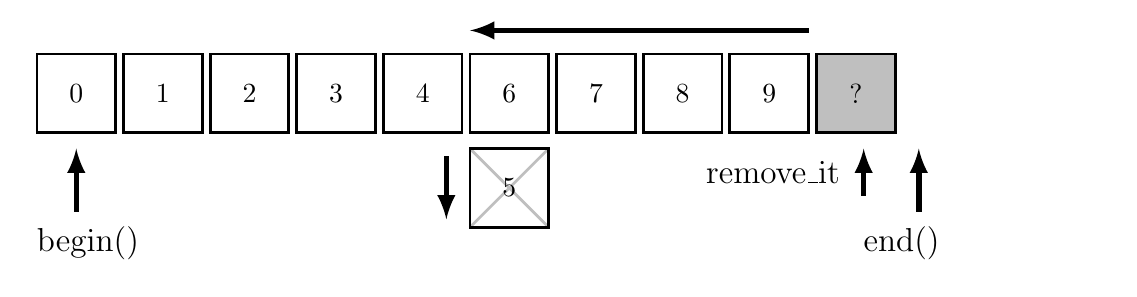
\begin{tikzpicture}
\draw[line width=2pt][-latex] (9.8,1.3) -- (5.5,1.3);
	
\foreach \x in {0,...,4} {
	\draw[line width=1pt] (1.1*\x,1) rectangle (1.1*\x+1,0) node[pos=.5] {\x};
}

\foreach \x [evaluate=\x as \index using int(\x+1)] in {5,...,9} {
	\draw[line width=1pt] (1.1*\x,1) rectangle (1.1*\x+1,0) node[pos=.5] {\index};
}

\foreach \x in {9} {
	\draw[fill=white!50!gray, line width=1pt] (1.1*\x,1) rectangle (1.1*\x+1,0) node[pos=.5] {?};
}

\draw[line width=2pt][-latex] (0.5,-1.0) -- (0.5,-0.2);
\draw[line width=2pt][-latex] (11.2,-1.0) -- (11.2,-0.2);
\draw[line width=2pt][-latex] (5.2,-0.3) -- (5.2,-1.1);
\draw[line width=2pt][-latex] (10.5,-0.8) -- (10.5,-0.2);

\draw[color=white!50!gray, line width=1pt] (1.1*5,-0.2) -- (1.1*5+1,-1.2); 
\draw[color=white!50!gray, line width=1pt] (1.1*5,-1.2) -- (1.1*5+1,-0.2);
\draw[line width=1pt] (1.1*5,-0.2) rectangle (1.1*5+1,-1.2) node[pos=.5] {5};

\node[text width=3cm, font=\large] at (1.5,-1.4) {begin()};
\node[text width=3cm, font=\large] at (12,-1.4) {end()};
\node[text width=3cm, font=\large] at (10.0,-0.5) {remove\_it};
\end{tikzpicture}

图3.2 移除一个元素
\end{center}

remove()函数的作用是:返回一个迭代器(remove\_it),指向移位的元素之后的第一个元素。end()迭代器保持在remove()操作之前的状态。为了进一步说明,若要使用remove\_if()删除所有偶数元素,结果如下所示:

\hspace*{\fill} \\ %插入空行
\begin{center}
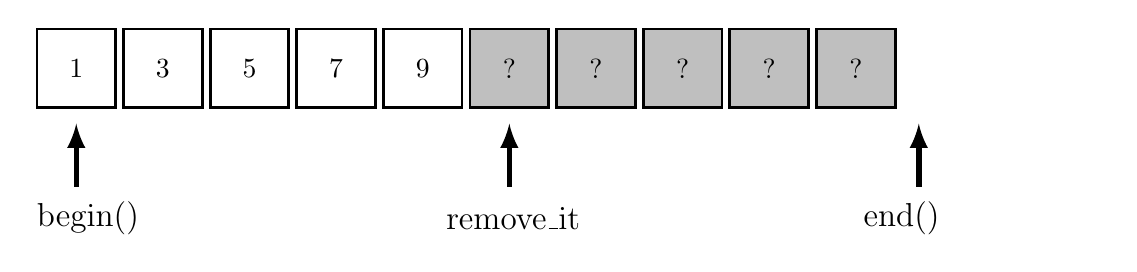
\begin{tikzpicture}

\foreach \x [evaluate=\x as \index using int(2*\x+1)] in {0,...,4} {
	\draw[line width=1pt] (1.1*\x,1) rectangle (1.1*\x+1,0) node[pos=.5] {\index};
}

\foreach \x [evaluate=\x as \index using int(\x+1)] in {5,...,9} {
	\draw[fill=white!50!gray, line width=1pt] (1.1*\x,1) rectangle (1.1*\x+1,0) node[pos=.5] {?};
}

\draw[line width=2pt][-latex] (0.5,-1.0) -- (0.5,-0.2);
\draw[line width=2pt][-latex] (6.0,-1.0) -- (6.0,-0.2);
\draw[line width=2pt][-latex] (11.2,-1.0) -- (11.2,-0.2);

\node[text width=3cm, font=\large] at (1.5,-1.4) {begin()};
\node[text width=3cm, font=\large] at (6.7,-1.4) {remove\_it};
\node[text width=3cm, font=\large] at (12,-1.4) {end()};
\end{tikzpicture}
	
图3.3 移除偶数元素后
\end{center}

本例中,剩下的就是5个奇数元素,后面跟着5个未定义值的元素。

然后,调用容器的erase()函数来擦除剩余的元素:

\begin{lstlisting}[style=styleCXX]
c.erase(remove_it, c.end());
\end{lstlisting}

容器的erase()函数使用remove\_it和end()迭代器调用,可以删除所有未定义的元素。

erase()和erase\_if()函数同时调用remove()函数和容器的erase()函数,以便一步执行erase-remove。




